\documentclass[a4paper,12pt]{article}
\usepackage{graphicx}
\usepackage{hyperref}
\usepackage{amsmath}
\usepackage{amsfonts}
\usepackage{afterpage}
\usepackage{amssymb}
\usepackage[nottoc]{tocbibind} % To include TOC, LOT, LOF in TOC
\usepackage{titlesec} % Package for custom section titles
\usepackage{tikz} % Package for drawing borders
\usetikzlibrary{shapes.geometric, arrows}
\usepackage{array}
\usepackage{caption} % Added package for adjusting caption spacing


% Customize the section formatting
\titleformat{\section}[block]
  {\normalfont\Large\bfseries}
  {\thesection}
  {1em}
  {}
\titlespacing*{\section}{0pt}{\baselineskip}{\baselineskip}


% TikZ styles
\tikzstyle{startstop} = [ellipse, minimum width=3cm, minimum height=1cm,text centered, draw=black, fill=white!30]
\tikzstyle{data} = [cylinder, shape border rotate=90, aspect=0.25, text width=4em, minimum height=4em, text centered, draw=black]
\tikzstyle{process} = [rectangle, minimum width=2cm, minimum height=1cm, text centered, draw=black]
\tikzstyle{subprocess} = [rectangle, minimum width=2.5cm, minimum height=1cm, text centered, draw=black, fill=white!10]
\tikzstyle{algobox} = [rectangle, rounded corners, minimum width=3cm, minimum height=0.75cm, text centered, draw=black]
\tikzstyle{arrow} = [thick,->,>=stealth]

% Adjust the spacing after the table caption
\captionsetup[table]{skip=10pt}

\begin{document}

% Cover Page
\begin{titlepage}

    \centering
    \Large
    \makebox[0pt]{\textbf{Khulna University of Engineering \& Technology}}\\
    \vspace{0.3in}
    \centering
    \Large
    \textbf{Course No:} CSE 4120 \\
    \textbf{Course Title:} Technical Writing and Seminar
    
    \vspace{0.3in}
    \Huge
    % Horizontal line
    \rule{\textwidth}{0.4pt}
    \textbf{Bangla Aspect-Based Sentiment Analysis}
    % Horizontal line
    \rule{\textwidth}{0.4pt}

    \vspace{0.5in}
    \Large
    \textbf{Submitted By:} \\
    Irhamul Islam \\
    Roll Number: 1907093 \\
    Department of Computer Science and Engineering \\
    Khulna University of Engineering \& Technology

    \vspace{0.5in}
    \textbf{Course Teachers:}

    \vspace{0.2in}
    \begin{minipage}{0.49\textwidth}
        \raggedright
        Dr. K. M. Azharul Hasan \\
        Professor \\
        Department of Computer Science and Engineering \\
        Khulna University of Engineering \& Technology
    \end{minipage}
    \hfill
    \begin{minipage}{0.49\textwidth}
        \raggedleft
        Sunanda Das \\
        Assistant Professor \\
        Department of Computer Science and Engineering \\
        Khulna University of Engineering \& Technology
    \end{minipage}

    \vfill
\end{titlepage}

% Abstract
\pagenumbering{roman}
\setcounter{page}{1}
%\addcontentsline{toc}{section}{Abstract}
\begin{abstract}
Sentiment analysis has been a very interesting topic for researchers as it is very useful in analyzing social media comments, online product review comments, etc. The usual sentiment analysis determines the emotion behind a text. Aspect-based analysis gives opinions based on different aspects of the content. At first, it extracts aspects from the sentence and then separates them based on their sentiment. In this study, I have reviewed three research papers that worked on aspect-based analysis for the Bengali language. They worked on the same dataset using different approaches. Solving this problem will be very helpful in various aspects and will create more research scope in the associated field.
\end{abstract}
\newpage

% Table of Contents
\pagenumbering{roman}
\setcounter{page}{2}
\tableofcontents
\newpage


% List of Tables
\setcounter{page}{4}
\listoftables
\newpage

% List of Figures
\setcounter{page}{5}
\listoffigures
\newpage

\clearpage

\pagenumbering{arabic}

% Introduction
\section{Introduction}
Number of users of social media is increasing day by day. Billions of people are writing posts, and comments and giving views about something. In recent years, people have become more involved to online shopping. During any pandemic situation like COVID-19, engagement in online shopping sites was heavy. The customers are constantly giving reviews or complaints about the product or service they're taking. Sentiment Analysis can analyze texts and give predictions of these large number of reviews, and comments.Thus giving narrow insight into whether the statement is positive, negative or neutral.So,sentiment analysis has become an important topic for researchers.\\[1\baselineskip]
Sentiment analysis labels the overall sentiment of a text. Whereas Aspect-Based Sentiment Analysis(ABSA) predicts the sentiment by detecting the aspects of a sentence.For example-\vspace{1em}
 
 \noindent\hspace{4cm}"Bangladesh is playing well."\vspace{1em}\\
For the above sentence, ABSA will predict the polarity positive under the aspect of sports.In ABSA, there are two steps - 1. term extraction and 2. sentiment classification means assigning the polarity.\\[1\baselineskip]
For the Bengali language, research on sentiment analysis is ongoing and improving gradually. There is a lack of research on topics like ABSA in the Bengali language. There are some shortcomings like - a lack of accurate or annotated datasets.\vspace{1em}\\
The reviewed research papers tried to improve the accuracy of aspect-based analysis(ABSA) in the Bengali language.In the first paper, a new approach called PSPWA(priority Sentence Part Weight Assignment) is introduced by Forhad\cite{first}. With CNN, this shows better results. In the second paper, they found that less pre-processing of data increases the accuracy\cite{second}. Both of the papers worked on the publicly available dataset. In the third paper, proposed a new version of the available dataset and named it BAN-ABSA\cite{third}. This dataset is annotated with aspects and corresponding sentiment. They also claimed that using Bi-LSTM performs better than CNN.\\[1\baselineskip]
ABSA is useful in many scenarios like social media comments or posts, online shopping reviews, or newspaper comments. At a glance, it can tell us the portion of positive or negative reviews from the large dataset. Thus bringing efficient analysis in the related field.

% Background/Problem Statement
\section{Background/Problem Statement}
Feedback from customers from social media, online reviews, newspaper comments, or customer online surveys is creating a large data every day. It is very painstaking and tough for humans to read all the content and understand the people's opinions from it.\\[1\baselineskip]
Unlike sentiment analysis,which gives an overall prediction, Aspect-Based analysis gives a far more better understanding.For example-{\vspace{1em}}

 \noindent\hspace{3cm}"Food is delicious but the service is poor."\vspace{1em}\\
It can be seen clearly that this comment of a restaurant review indicates positive feedback for the food but a negative opinion of the service in the same sentence. In usual overall prediction, it will show the opinion is bad of a customer. But this neglects the fact that the customer was happy with the food. So, there are two aspects-food and service. Based on that, if sentiment is analyzed, that will give a better understanding. This is Aspect-Based Sentiment Analysis in short ABSA.\\[1\baselineskip]
There are four sub-tasks for ABSA mentiond in SemEval\cite{semeval}-  \\[1\baselineskip]
\textbf{Aspect Term extraction}\\[1\baselineskip]
Detecting a list of particular aspect terms from a sentence. \\[1\baselineskip]
\textbf{Aspect Term Polarity}\\[1\baselineskip]
This assigns a label like positive, negative, or neutral in various aspect terms that have been extracted. \\[1\baselineskip]
\textbf{Aspect Category Detection}\\[1\baselineskip]
There are some predefined sets of aspect categories. Comparing with that, identifying the aspect categories of the given sentence.\\[1\baselineskip]
\textbf{Aspect Category Polarity}\\[1\baselineskip]
After detecting the category, determines the polarity for each aspect.

% Review of Literature
\section{Review of Literature}
ABSA in the Bangla language is first introduced in 2018,done by Rahman and Dey\cite{rahman2018datasets}.The dataset is made publicly available.Liu,B. first introduced ABSA.He first described it's procedures and sub-tasks.\cite{liuABSA}.\newline
For opinion expression extraction,Cahyadi built an ABSA model using Bi-LSTM and Convolutional Neural Network(CNN) for sentiment polarity\cite{cahyadi2018aspect}.Nandan proposed that lexicon-based presents less performance than machine learning techniques\cite{nandal2019aspect}.Nazir done a research to find out the challenges of ABSA\cite{challenges}.\newline
Based on stacked auto-encoders boidini developed a ABSA model that achieved better f1-score than Rahman and Dey's research of 2019\cite{encoder}.Based on Recurrent Neural Network(RNN), Wahid did a study of sentiment analysis in Bangla text\cite{wahid2019cricket}.\newline
In SemEval, ABSA's task is divided into four subtasks\cite{semeval}.In aspect extraction,a rule-based approach has been propsed from product reviews\cite{rule-based}.In a reserach,the authors introduced two new corpora in Czech language to solve ABSA\cite{czech}.\newline
To implement ABSA,clause level classification can give significant performance for both tasks\cite{clauselevel}.Among many created datasets for ABSA,one is named Sentihood containing 5215 sentences collected from yahoo\cite{saeidi2016sentihood}.In Hindi,a dataset for sentiment analysis is created containing 5412 comments of Hindi product reviews\cite{hindi}.
% Methodology
\section{Methodology}
\subsection{Bangla Aspect-Based Sentiment  Analysis Based on Corresponding Term Extraction}
\subsubsection{Dataset Collection}
Dataset used in this research is a publicly available dataset first implemented in ABSA by Rahman and Dey\cite{rahman2018datasets}.Cricket and Restaurant are two datasets of Bangla language .These generally contains the feedback of people on this topics.Link for the dataset-\url{https://github.com/atik-05/Bangla_ABSA_Datasets}
\newpage
\begin{table}[h!]
    \centering
    \caption{Overall summary of datasets}
    \vspace{0.5cm}
    \begin{tabular}{|c|c|c|}
        \hline
        & \textbf{Cricket} & \textbf{Restaurant} \\
        \hline
        \textbf{No. of Sentence} & 2979 & 2059 \\
        \hline
        \textbf{Aspect Category} & Batting, Bowling, Team & Food, Service, \\
                                 & Management, Team, Other & Price, Ambiance, \\
                                 & & Miscellaneous \\
        \hline
        \textbf{Aspect Polarity} & Positive (19\%) & Positive (59\%) \\
                                 & Negative (72\%) & Negative (23\%) \\
                                 & Neutral (9\%) & Neutral (6\%) \\
                                 & & Conflict (12\%) \\
        \hline
    \end{tabular}
\end{table}
\subsubsection{Data Preprocessing}
To make the dataset useable for the model, in pre processing step, unnecessary characters are removed. Here, punctuation and numerical words such as Dari(' \textbar '), Comma(','), etc are eradicated as these carry no significant impact on the result.
\subsubsection{Feature Enginneering}
For better performance of any machine learning model, feature engineering plays an effective role. Using Term Frequency and Inverse Document Frequency(TF-IDF), the dataset has been tokenized.\\
Constant features do not affect target outputs. These values are negligible. That's why, these features are removed from the numbered matrix.\\
Correlated features are influenced by common mechanisms. Highly correlated features give redundant information. These values were also removed from the numbered matrix.\\
For removing constant features and correlated features, the threshold values were 0.005 and 0.75 respectively.
\subsubsection{Priority Sentence Part Weight Assignment(PSPWA)}
NOUNS of a sentence is focused on extracting aspect terms. It is considered that NOUNS are priority words.In any sentence, the portion holding a NOUN is the priority sentence part.
\newpage
\begin{figure}[h]
    \centering
    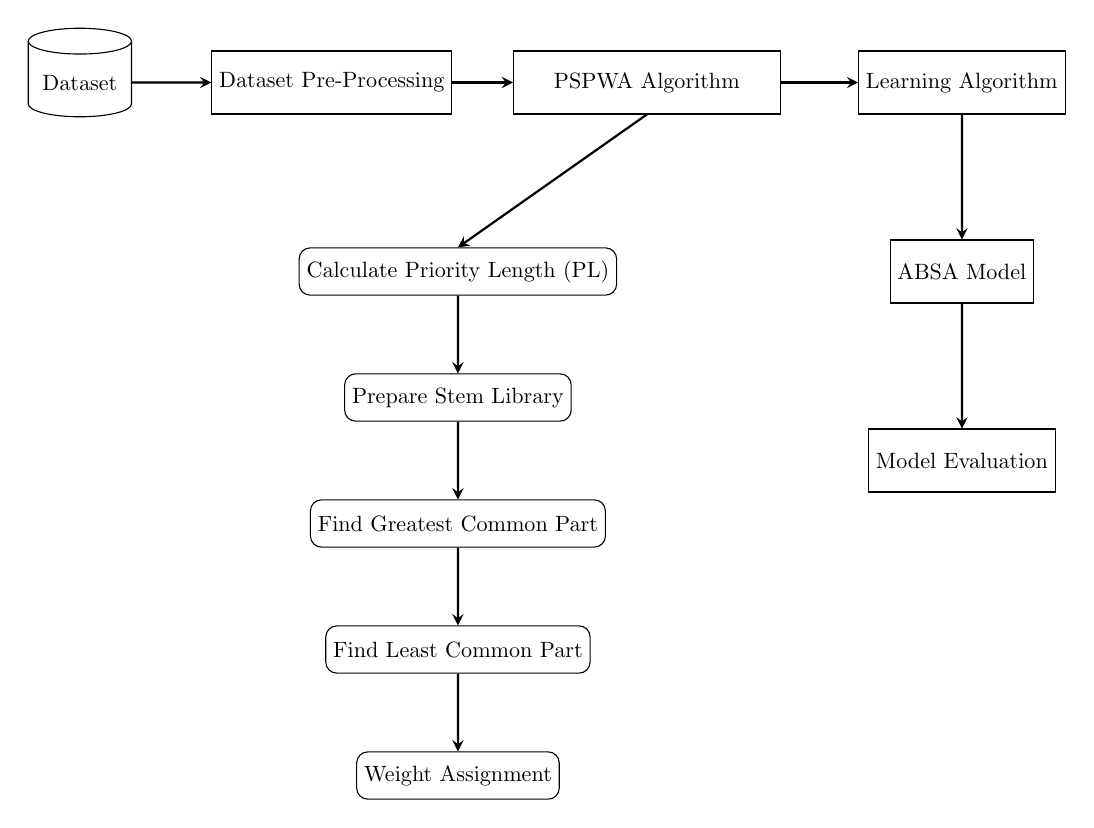
\begin{tikzpicture}[node distance=2cm,scale=0.8, transform shape]

    % Nodes
    \node (dataset) [data] {Dataset};
    \node (preprocess) [process, right of=dataset, xshift=2cm] {Dataset Pre-Processing};
    \node (pspwa) [process, right of=preprocess, xshift=3cm, text width=4cm] {PSPWA Algorithm};
    \node (learning) [process, right of=pspwa, xshift=3cm] {Learning Algorithm};
    \node (absa) [process, below of=learning, yshift=-1cm] {ABSA Model};
    \node (evaluation) [process, below of=absa, yshift=-1cm] {Model Evaluation};

     \node (calculate) [algobox, below of=pspwa, yshift=-1cm, xshift=-3cm] {Calculate Priority Length (PL)};
    \node (stem) [algobox, below of=calculate] {Prepare Stem Library};
    \node (greatest) [algobox, below of=stem] {Find Greatest Common Part};
    \node (least) [algobox, below of=greatest] {Find Least Common Part};
    \node (weight) [algobox, below of=least] {Weight Assignment};

    % Arrows
    \draw [arrow] (dataset) -- (preprocess);
    \draw [arrow] (preprocess) -- (pspwa);
    \draw [arrow] (pspwa) -- (learning);
    \draw [arrow] (learning) -- (absa);
    \draw [arrow] (absa) -- (evaluation);

    \draw [arrow] (pspwa.south) -- (calculate.north);
    \draw [arrow] (calculate) -- (stem);
    \draw [arrow] (stem) -- (greatest);
    \draw [arrow] (greatest) -- (least);
    \draw [arrow] (least) -- (weight);

    \end{tikzpicture}
    \caption{Diagram for proposed method for first paper}
    \label{fig:pspwa}
\end{figure}
\begin{enumerate}
\item \textbf{Priority Length (PL)}: \\
    To find out the priority part, an equation is applied. This returns an integer value. The equation looks like below.
    
    \begin{equation}
        \text{PL} = \min(\text{LEN}(\text{SENTENCE}), 3) + \frac{\text{LEN}(\text{SENTENCE})}{3} - 1
    \end{equation}
   
    \item \textbf{Stem/ Root Form of Verb}:\\
    Roots are the base from of the words.A suffix or prefix can be added to that word but expresses the same meaning.
    \item \textbf{Greatest Common Part \& Least Common Part}\\
   The greatest Common Part is considered to be the largest frequency sentence part of the stem. It is the priority part and the Least Common Part is the least frequency sentence part of the stem. It is not a priority part.
   \newpage
    \item \textbf{Weight Assignment}:
    \begin{itemize}
        \item Initially,weight is zero for each word.
        \item Convert the words of sentence to stem.
        \item If any word is present within the priority part, increase one
        \item If sentence part of word matches with GCP of stem, increase one
        \item If sentence part of word and GCP both are priority part, increase one
        \item If sentence part of word don’t match with LCP, increase one
        \item If weight of word is greater than zero , then the weight is being multiplied  with corresponding value of the word in TF-IDF matrix.
        \item Then the result is replaced with the corresponding value in TF-IDF matrix. The equation looks like this-\\
        \begin{equation}
       Matrix_{i,j} = Matrix_{i,j} \times W_{i,j} \quad ; \quad \text{if } W_{i,j} > 0 W_{i,j} > 0
        \end{equation}
    \end{itemize}
    \item \textbf{Normalization}:\\
    Min-Nax classifier is applied as a normalization technique to transform all features in a suitable range.Equation of Min-Max classifier is given below - \\
    \begin{equation}
    \text{Matrix}_{i,j,\text{scaled}} = \frac{\text{Matrix}_{i,j} - \text{MIN}(\text{Matrix}_{i,j})}{\text{MAX}(\text{Matrix}_{i,j}) - \text{MIN}(\text{Matrix}_{i,j})}
    \end{equation}
\end{enumerate}

\subsubsection{Algorithm analysis}
Several learning algorithms have been used to implement the proposed method. Methods like K-nearest neighbor (KNN), Support Vector Machine (SVM), Linear Regression (LR), Random Forest (RF), and Convolutional Neural Network (CNN) have been employed. The values of the parameters are given below. These values are determined by trying many experimental values.

\begin{table}[h!]
    \centering
    \caption{Parameter list of CNN and supervised learning algorithms}
    \begin{tabular}{|c|m{10cm}|}
    \hline
    \textbf{Classifier} & \textbf{Parameter} \\
    \hline
    KNN & No of neighbors = 3, Metric = Euclidean \\
    \hline
    SVM & Max iterations = 1000, Multi class = 'ovr' \\
    \hline
    LR & Solver = 'sag', Max iterations = 150 \\
    \hline
    RF & Criterion = 'gini', No of estimators = 150 \\
    \hline
    CNN & Optimizer = 'adam', Learning rate = 0.0005, Batch Size = 100, Epochs = 20, Convolution Activation = 'relu', Dense Activation = 'softmax', Loss Function = 'crossentropy' \\
    \hline
    \end{tabular}
\end{table}
\textbf{CNN Architecture}: \\\hspace*{1cm}Two steps - 1.Feature extraction and 2.Classification
    \begin{itemize}
        \item Feature extraction is a combination of convolutional and pooling layers.
        \item The first CONV layer identifies low-level features.It becomes adaptable to high-level features if more layers are added.
        \item The Classification step, based on information on CONV layers, classifies output.
        \item Learning rate of 0.0005 using ADAM as it converges faster\cite{ADAM}
        \item Cross-entropy has been used as a loss function
        \item RELU used as a convolutional activation function
        \item Proposed CNN has seven layers.
        \item The output of the TF-IDF numbered matrix will be input for the CONV layer. Here, padding remains the same. 
    \end{itemize}
The dataset is divided into two sets test data and train data. Giving 80\% of the dataset to the training dataset and 20\% to the testing dataset.
\subsection{Aspect Based Sentiment Analysis in Bangla Dataset Based on Aspect Term Extraction}
\subsubsection{Dataset Collection}
The publicly available dataset for ABSA by Rahman and Dey of 2018 is used for analysis\cite{rahman2018datasets}. This dataset is created for the first time in Bengali.Link for the dataset-\url{https://github.com/atik-05/Bangla_ABSA_Datasets}\\
In the Cricket dataset, humans annotated the comments in five different aspects -bowling, batting, team, team management, and others. The restaurant dataset is translated into Bengali from the SemEval English dataset\cite{semeval}. Here also, five aspects-Food, Price, Service, Ambiance, and Miscellaneous.The datset overview can be seen in Table 1.
%add the diagram here
\begin{figure}[h!]
    \centering
    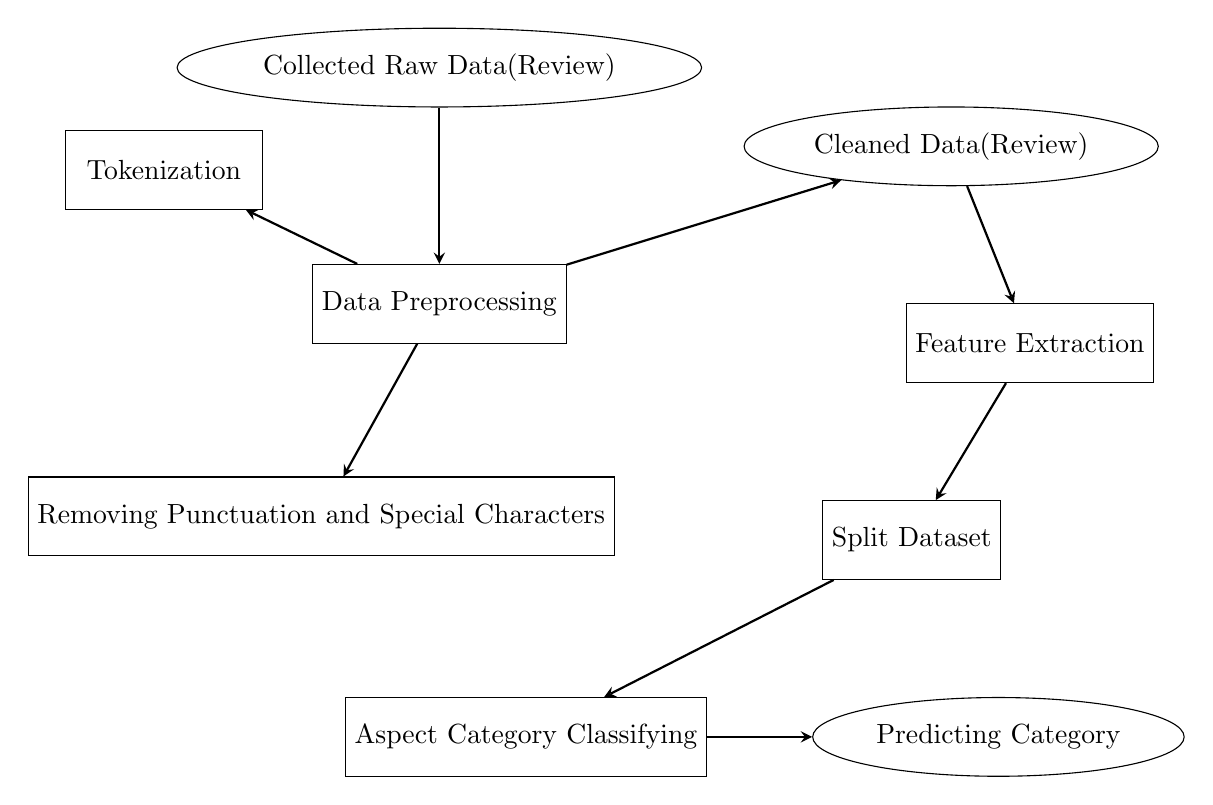
\begin{tikzpicture}[node distance=2cm]
        % Nodes
        \node (start) [startstop] {Collected Raw Data(Review)};
        \node (preprocess) [process, below of=start, yshift=-1cm] {Data Preprocessing};
        \node (removepunc) [subprocess, below of=preprocess, yshift=-0.7cm, xshift=-1.5cm] {Removing Punctuation and Special Characters};
        \node (tokenization) [subprocess, left of=preprocess, yshift=1.7cm, xshift=-1.5cm] {Tokenization};
        \node (cleaned) [startstop, right of=start, xshift=4.5cm, yshift=-1cm] {Cleaned Data(Review)};
        \node (feature) [process, below of=cleaned, yshift=-0.5cm,xshift=1cm] {Feature Extraction};
        \node (split) [process, below of=feature, yshift=-0.5cm,xshift=-1.5cm] {Split Dataset};
        \node (classifying) [process, below of=split, yshift=-0.5cm,xshift=-4.9cm] {Aspect Category Classifying};
        \node (predicting) [startstop, right of=classifying, xshift=4cm] {Predicting Category};

        % Arrows
        \draw [arrow] (start) -- (preprocess);
        \draw [arrow] (preprocess) -- (removepunc);
        \draw [arrow] (preprocess) -- (tokenization);
        \draw [arrow] (preprocess) -- (cleaned);
        %\draw [arrow] (tokenization.east) |- (cleaned.north);
        %\draw [arrow] (removepunc.east) |- (cleaned.north);
        \draw [arrow] (cleaned) -- (feature);
        \draw [arrow] (feature) -- (split);
        \draw [arrow] (split) -- (classifying);
        \draw [arrow] (classifying) -- (predicting);
    \end{tikzpicture}
    \caption{Proposed Model of Corresponding Term Extraction}
    \label{fig:flowchart}
\end{figure}

\subsubsection{Data Preprocessing}
Data preprocessing is a significant step in doing natural language processing tasks. The given dataset may contain some redundant characters that don't add any value to the final output or it may contain some information that may add complexity for the model analysis.\\

Here,text data is reduced by various steps which made the input size smaller.The steps are -
\vspace{0.2cm}
\begin{enumerate}
    \item \textbf{Removing special characters}:\\
    Special characters lead to ambiguity in the model often. That's why, they are removed from the dataset. Otherwise, unnecessary complexity would have been created.
    \vspace{0.5cm}
    \item \textbf{Removing punctuations}: \\
    Removing punctuations is a very well-known preprocessing step.As there is change even in punctuation from language to language, Punctuations were removed.
\end{enumerate}

\subsubsection{Feature Extraction}
In this procedure, texts have been converted to numeric form to use them as a feature. The procedure follows – \\
\begin{enumerate}
    \item \textbf{BOW}:\\
    To train any statistical algorithm using machine learning, the dataset has to be in numeric form.To ensure the functionality, the texts are converted to numbers.Bag Of Words can be used as a technique to implement this. This reflects the frequency of words in a textual content\cite{BOW}.
    \vspace{0.3cm}
    \item \textbf{TF-IDF} : \\
    It is evident from the name that it contains two words –TF and IDF. The first one means Term Frequency and the latter means Inverse Document Frequency.\\
    TF counts the frequency of a word in a content.IDF indicates the importance and weight of that word..
\end{enumerate}
    Equation for TF and IDF is given below:

% Term Frequency (TF)
\begin{equation}
\text{TF}(t) = \frac{\text{Number of times term } t \text{ appears in a document}}{\text{Total number of terms in the document}}
\end{equation}

% Inverse Document Frequency (IDF)
\begin{equation}
\text{IDF}(t) = \log_e \left( \frac{\text{Total number of documents}}{\text{Number of documents with term } t \text{ in it}} \right)
\end{equation}
Sklearn library\cite{pedregosa2011scikit} is used which contains the TFiDfVectorizer class. This is used to convert the feature into TF-IDF feature vectors. limitation of maximum features was set to 2500.
\vspace{0.5cm}
\subsubsection{Algorithm Analysis}
Several trials and errors have to be faced before finalizing which machine learning algorithm will be used to determine the outcome. This is a very rigorous process as the algorithm efficiency varies from dataset to dataset. The algorithms used in previous research have also been considered. The algorithms mentioned below are selected finally to classify.

\begin{enumerate}  
    \item To compare with the result of Rahman \& Dey\cite{rahman2018datasets}:
    \begin{itemize}
        \item SVM (Support Vector Machine)
        \item RF (Random Forest)
        \item KNN (K-Nearest Neighbor)
    \end{itemize}
    \item Additionally used:
    \begin{itemize}
        \item LR (Logistic Regression) \cite{LR}
        \item NB (Naïve Bayes)
    \end{itemize}
\end{enumerate}
\vspace{0.5cm}
Logistic Regression works best for prediction and classification problems. It is a suitable regression analysis to work on binary variables. To find the relationship between one dependent variable and several independent variables, LR was used here.\\
Naïve Bayes has good efficiency for predictive modeling. It usually assumes that every input is independent. NB is selected as it is less affected by data scarcity. It is often used in sentiment analysis tasks.\\
The dataset is divided as 80\% for training and 20\% for testing.

\subsubsection{Languages and Tools}
\begin{itemize}
    \item Python 3 (Jupyter Notebook) in Anaconda
    \item Python modules: scikit-learn\cite{pedregosa2011scikit}
    \item NLTK (A leading platform for building Python programs)\cite{nltk}
\end{itemize}
\subsection{BAN-ABSA: An Aspect-Based Sentiment Analysis dataset for Bengali and it’s baseline evaluation}
\subsubsection{Data Collection}
There has always been a lack of a proper dataset for the Bengali language in the field of aspect-based sentiment analysis. In past research, two datasets were present but they contained very few comments.

\vspace{0.5cm}

Here, a new high-standard dataset is created.it is named BAN-ABSA. has 9009 comments from many Bangali news sites.The dataset has sentences containing :
    \begin{itemize}
    \item Aspects:
    \begin{itemize}
        \item Politics
        \item Sports
        \item Religion
        \item Others
    \end{itemize}
    \item Polarity:
    \begin{itemize}
        \item Positive 
        \item Negative
        \item Neutral
    \end{itemize}
\end{itemize}

\vspace{0.5cm}

Comments were collected from several news portals where people expressed their opinions and views about any particular matter. This could be comments or posts. The popular news sites were selected as they had more engagement of people.Data collection overview:
    \begin{itemize}
    \item Daily Prothom Alo: 16735 comments
    \item Daily Jugantor: 14389 comments
    \item Kaler Kantho: 8062 comments
\end{itemize}
These 39186 comments were collected.
\subsubsection{Annotating Data}
After collecting the comments, they were preprocessed. Multi-lined comments have been removed or multi-lined comments trimmed into a singe-line comments. Emojis were also removed.\newline
In the annotating phase, the data was divided into three parts. They were distributed among 9 annotators. Each comment was annotated by 3 annotators. They analyzed the data for aspect and polarity. The comments can be in one of the three aspects: politics, religion, and sports. If the comment
that doesn't match with the mentioned aspects, goes to the other aspect.
The polarity can be either positive, negative, or neutral. Majority voting was followed to avoid any contradiction.\newline
For example, to do aspect annotation, say two annotators marked a sentence as politics, and one annotator marked it as Religion
aspect. From majority voting, it was decided to annotate this comment as
having a political aspect. No tie situation was faced.\newline
Finally, 9009 comments were labeled. The dataset contains
four aspects and 3 polarities. The dataset was created such it maintains balance. Like, in the case of news, people write no comments for good news. On opposite, a lot of comments can be found on a post about any negative incident.
\begin{figure}[h!]
    \centering
    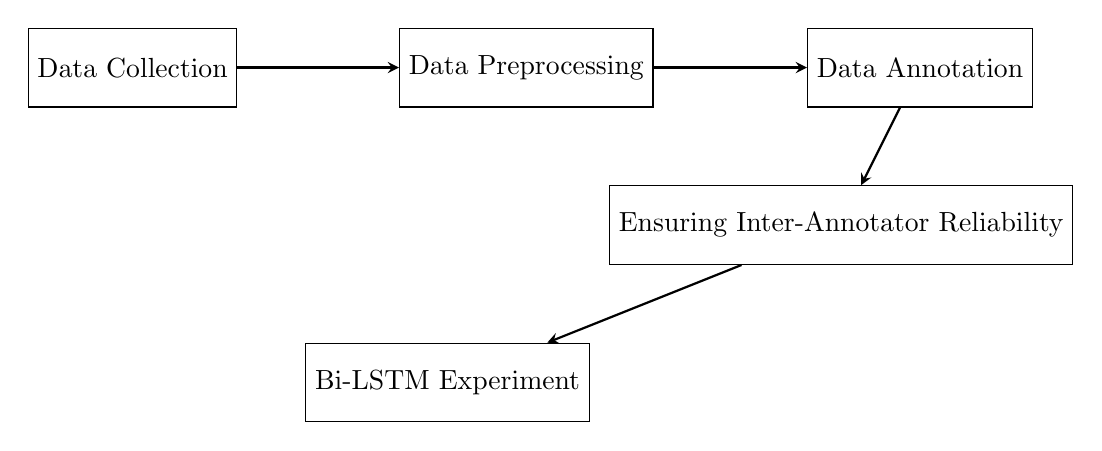
\begin{tikzpicture}[node distance=2cm,scale=0.9]

    % Nodes
    \node (collection) [process] {Data Collection};
    \node (preprocessing) [process, right of=collection, xshift=3cm] {Data Preprocessing};
    \node (annotation) [process, right of=preprocessing, xshift=3cm] {Data Annotation};

    \node (reliability) [process, below of=annotation, xshift=-1cm] {Ensuring Inter-Annotator Reliability};
    \node (experiment) [process, left of=reliability, yshift=-2cm,xshift=-3cm] {Bi-LSTM Experiment};

    % Arrows
    \draw [arrow] (collection) -- (preprocessing);
    \draw [arrow] (preprocessing) -- (annotation);
    \draw [arrow] (annotation) -- (reliability);
    %\draw [arrow] (collection) -- (experiment);
    \draw [arrow] (reliability) -- (experiment);
    %\draw [arrow] (zipf) -- (experiment);

    \end{tikzpicture}
    \caption{Proposed Model for BAN-ABSA}
    \label{fig:flowchart}
\end{figure}
\subsubsection{Dataset Analysis}
To ensure annotator's reliability, Intra-class Correlation Coefficient (ICC) was calculated.It came 0.77.\newline
Zipf’s law was also applied \cite{powers1998applications} in our dataset.The law states that, the collection frequency (cfi) of the ith most common term in the
dataset should be proportional to 1/i .
\begin{equation}
c_{f_i} \propto \frac{1}{i}
\end{equation}
\subsubsection{Experiment With Bi-Directional Long Short Term Memory}
After creating the benchmark dataset, BAN-ABSA, which can be used for both the sub-tasks: aspect extraction and sentiment classification.\newline
In the pre-processing phase, The comments were removed containing English words. All the punctuation marks were removed. Then, the data was tokenized.\newline
Some deep neural network models and some traditional supervised machine learning models were used to complete this task. In the experiment, Bi-LSTM showed good performance achieving the highest f1-score.
\begin{itemize}
    \item \textbf{Bi-Directional Long Short Term Memory}\newline
    Recurrent Neural Networks (RNN) show good results and they are highly used in text classification.But, RNN has a vanishing gradient problem.To resolve this issue, LSTM was proposed \cite{lstm}.\newline
    In LSTM, information can only be transferred in forward states. At any time, the state is dependent only on past information. But forward information may also be required in some cases.\newline
    BiLSTM is introduced to solve this problem. BiLSTM’s architecture consists of two hidden, opposite-direction LSTM layers to completely hold the input context.Regular RNN’s state neurons are split into two parts.One part captures features of the past and uses forward states.The other one takes features of the opposite direction and uses backward states\cite{bilstm}.
\end{itemize}


% Result Analysis
\section{Result Analysis}
F1-score as an evaluation matrix is presented to compare the three papers for result accuracy and to evaluate model performance. The papers used 
various learning algorithms. Here, not all algorithms are followed the same in all papers. Like, Forhad\cite{first} used CNN but Haque et al.\cite{second} did not.\newline
The True Positive (TP), True Negative (TN), False Positive (FP), and False Negative (FN) are four parameters to measure the terms f1-score, precision, and recall.\newline
\begin{equation}
\text{Precision} = \frac{TP}{TP + FP}
\end{equation}

\begin{equation}
\text{Recall} = \frac{TP}{TP + FN}
\end{equation}

\begin{equation}
\text{F1-score} = \frac{2 \cdot \text{Precision} \cdot \text{Recall}}{\text{Precision} + \text{Recall}}
\end{equation}
In the following table,the first two papers are compared .Both Forhad\cite{first} and Haque et al.\cite{second}worked on the same dataset.
\begin{table}[h!]
    \centering
    \begin{tabular}{|c|c|c|c|}
        \hline
        \textbf{Method} & \textbf{Dataset} & \textbf{Paper 1} & \textbf{Paper 2} \\
        \hline
        SVM & Cricket & 0.48 & 0.35 \\
        \hline
        KNN & Cricket & 0.31 & 0.27 \\
        \hline
        RF & Cricket & 0.41 & 0.37 \\
        \hline
        LR & Cricket& 0.48 & 0.34 \\
        \hline
        NB & Cricket & 0.39 & 0.18 \\
        \hline
        CNN & Cricket & 0.59 & not applied \\
        \hline
    \end{tabular}
    \caption{F1-Score comparison on cricket dataset}
    \label{tab:example}
\end{table}

It can be seen that Forhad\cite{first} performs better than Haque et al.\cite{second} significantly using the method SVM and LR.\newline
These two papers also worked on the restaurant dataset.Table 4 shows the comparison.
\begin{table}[h!]
    \centering
    \begin{tabular}{|c|c|c|c|}
        \hline
        \textbf{Method} & \textbf{Dataset} & \textbf{Paper 1} & \textbf{Paper 2} \\
        \hline
        SVM & Restaurant & 0.52 & 0.39 \\
        \hline
        KNN & Restaurant & 0.39 & 0.38 \\
        \hline
        RF & Restaurant & 0.35 & 0.35 \\
        \hline
        LR & Restaurant & 0.44 & 0.43 \\
        \hline
        NB & Restaurant & 0.34 & 0.17 \\
        \hline
        CNN & Restaurant & 0.67 & not applied \\
        \hline
    \end{tabular}
    \caption{F1-Score comparison on restaurant dataset}
    \label{tab:example}
\end{table}

Here also , Forhad\cite{first} performed better than Haque et al.\cite{second}.\newline
The third paper created a new benchmark dataset named BAN-ABSA\cite{third}.They worked on that showing a significant good result.The following table shows the f1-score for the corresponding algorithms.
\begin{table}[h!]
    \centering
    \begin{tabular}{|c|c|c|}
        \hline
        \textbf{Method} & \textbf{Dataset} & \textbf{Paper 3} \\
        \hline
         SVM & BAN-ABSA & 0.69\\
        \hline
        KNN & BAN-ABSA & 0.47 \\
        \hline
        RF & BAN-ABSA & 0.65 \\
        \hline
        CNN & BAN-ABSA & 0.75 \\
        \hline
    \end{tabular}
    \caption{F-1 score table for BAN-ABSA}
    \label{tab:example}
\end{table}
This paper shows a far better f1-score than the rest two in aspect-based sentiment analysis.Apart from the methods mentioned in the table, they also used LSTM and Bi-LSTM.\newline
Using LSTM and  Bi-LSTM for aspect extraction on the proposed dataset, they achieved f1-score of 77.24 and 79.38 respectively. 
% Findings and Recommendations
\section{Findings and Recommendations}
From this rigorous study of three research papers solving the same problem, some insights have been gained.They are mentioned below:\newline
\begin{itemize}
        \item Feature engineering reduces dataset shape.This phase excludes the constant and correlated features.The refined dataset is more suitable for the learning model.
        \item The PSPWA technique mentioned in the first paper by Forhad\cite{first} replaced the TD-IDF score of the numbered matrix by assigning a new weight.
        \item Overfitting is an issue for tasks like sentiment analysis. This problem can be solved by adding more training samples or reducing features.\newline
        In the feature engineering phase, the dataset is already reduced by eliminating some redundant data. As the first two papers,Forhad\cite{first},Haque et al.\cite{second} used publicly available datasets, adding more samples could not be implemented.\newline
        The third paper,BAN-ABSA\cite{third} created its own high standard dataset which showed better result
        \item In the first paper,Forhad\cite{first}, applying PSPWA in the data pre-processing step has helped to gain a better F1-Score than previous studies.

        \item The second paper,Haque et al.\cite{second} has provided better results by reducing some preprocessing steps. This less preprocessing leads to better F1 scores in both datasets (Restaurant and Cricket).\newline
        Aspect category extraction is a multi-label classification problem [5] where one sentence might carry several categories.That's why, the proposed method here may skip some aspect categories.There is room for improvements.\newline
        One solution can be by training the dataset using POS tagging.
        \item As for the learning algorithms, several algorithms have been used to evaluate the proposed model in all three papers. In general, it can be said that CNN and LR performed better than the other methods.\newline
        Additionally, for aspect term extraction LSTM and Bi-LSTM are used in the third paper,BAN-ABSA\cite{third}.This showed far better accuracy than other methods.
        \item The dataset plays a vital role in aspect-based sentiment analysis. Rather than the publicly available dataset, BAN-ABSA\cite{third} showed far better performance. 
\end{itemize}

\vspace{0.7cm}


After analyzing the findings by studying the three research papers, I highly recommend the third paper, \textbf{BAN-ABSA}\cite{third} for the best performance among those. It showed good results both in terms of aspect extraction and polarity of sentence detection.I propose the Bi-LSTM architecture to be used in Aspect Based Sentiment Analysis. The main reasons are :
\begin{itemize}
        \item Creating a high-standard dataset for the Bengali language.
        \item Achieving high accuracy for aspect extraction by using Bi-LSTM.
        \item Better f1-score than the remaining papers in sentiment analysis.    . 
\end{itemize}

% Addressing Course Outcomes and Program Outcomes
\section{Addressing Course Outcomes and Program Outcomes}

The course titled "Technical Writing and Seminar" has outcomes in the following way:

\begin{itemize}
    \item \textbf{Problem Analysis}:\\
    In this course, a problem was analyzed. To implement this, three research papers were selected.Each of them tried to solve the problem with different approaches.the papers were studied thoroughly and an understanding was developed of the methodology or the solution approach. By doing so, it is learned how to think of different solutions for a particular issue.

    \item \textbf{Ethics}:\\
    Throughout this course, ethical values were maintained. For example, this report, it was tried to maintain the highest level of integrity which means - not copying other works or giving credit to someone whose work has been borrowed.

    \item \textbf{Individual and Teamwork}:\\
    The task of problem analysis was done individually. By analyzing three papers, it is learned that how to study research papers and make a review of those papers individually.\newline
    Throughout the course, in many cases, teamwork was involved. In regular sessionals, tasks were given. Sometimes, they were solved collaboratively with the help of others. Thus, ensuring teamwork ability.

    \item \textbf{Communication}:\\
    Communication skill was developed by giving effective presentations, communicating with course teachers regarding engineering activities, etc. Designing documents or reports also helped to furnish one's communication ability.
\end{itemize}

    
    


% Addressing Complex Engineering Activities
\section{Addressing Complex Engineering Activities}
The following attributes of Complex Engineering Activities was gained:

\begin{itemize}
    \item \textbf{Range of resources}:\\
    In analyzing a problem, resources can vary for a large range. Information is needed to check the validity of the research papers. To understand the studies, other knowledge was gained from various sources. This report is written using latex which is also a resource.
    \item \textbf{Level of interaction}:\\
    While understanding the problem, interaction to different people or between different domains of topics happened.

    \item \textbf{Innovation}:\\
    The three research papers tried to solve the problem in their unique way. Thus, leading to an innovation.

    \item \textbf{Consequences for society and the environment}:\\
    Solving this problem will be impactful for society,Sentiment analysis has various applications in social media monitoring in online shopping reviews, etc.
    \item  \textbf{Familiarity}:\\
    There were some research studies done on this topic before. The papers mentioned tried to improve the solution by proposing a new methodology.Although there are familiarity, each of the papers contributes in a different way.
\end{itemize}

% Conclusion
\section{Conclusion}
In this study, three research papers were discussed solving the problem of aspect-based sentiment analysis. Each paper proposed different approaches to solve this issue.\newline
The ABSA model works into two parts - 1. aspect terms extraction and
2. aspect polarity determination.A new technique named PSPWA is introduced for extracting aspect terms which has improved the F1-score.\newline
With less preprocessing, gives better outputs for aspect extraction. Two traditional steps can be used to clean data.With a proper dataset, this result can be improved.The BAN-ABSA dataset\cite{third} is a significant contribution in research in this field.\newline
Resource barriers hindered many researchers from doing work on Bengali ABSA. BAN-ABSA\cite{third} can be used in further ABSA tasks and create more research scope.\newline
Sentiment analysis is useable for various cases like spam review or comment detection and fraud app detection. This can help to make better business decisions also improve cyber security.\newline
In the future,  more advanced techniques of deep learning can be applied in NLP for ABSA. Continuous exploration may lead to finding better learning techniques. Also, the Bangla POS tagger can be explored to train the model in aspect term extraction and train classifier.\newline
The found results are not too high compared to English ABSA. Modifications need to be made to improve the overall performance. In the Bengali language, this type of research needs to be done more as there is scope for improvements.

% Bibliography
\bibliographystyle{plain}
\bibliography{ref}

\newpage
% Manually add an entry to the Table of Contents
\addcontentsline{toc}{section}{Publication Details}

\begin{table}[h]
    \centering
    \begin{tabular}{|p{1cm}|p{4cm}|p{3cm}|p{2cm}|p{2cm}|p{1cm}|}
        \hline
        SL No. & Title & Authors & Publishers & Source & Year  \\
        \hline
         1 & Bangla Aspect-Based Sentiment Analysis Based On Corresponding Term Extraction\cite{first} & Forhad An Naim & IEEE & International Conference on ICT & 2022 \\
        \hline
        2 & Aspect Based Sentiment Analysis in Bangla Dataset Based on Aspect Term Extraction\cite{second} & Sabrina, Tasnim, Asif, Shohel, Biplod, Himu & Springer & Second EAI International Conference & 2023 \\
        \hline
        3 & BAN-ABSA: An Aspect-Based Sentiment Analysis Dataset for Bengali and its Baseline Evaluation\cite{third} & Masum, Junaed, Ayesha, Saiful & Springer & Proceedings of International Joint Conference on Advances in Computational Intelligence & 2024 \\
        \hline
    \end{tabular}
    \caption{Publication Details}
    \label{tab:publication_details}
\end{table}



\end{document}

\end{document}
